\documentclass{standalone}
\usepackage{tikz}
\usetikzlibrary{patterns, angles}
\usepackage{circuitikz}

\begin{document}
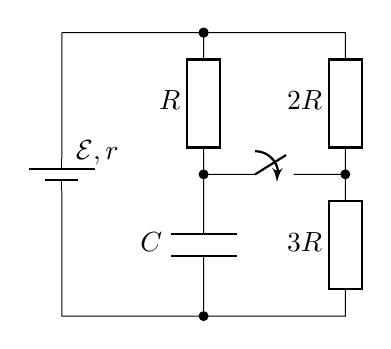
\begin{tikzpicture}[european, scale=0.9]
	\draw (0,4) to [battery1] (0, 0) to [short, -*] (2,0) to [capacitor=$C$, -*] (2,2) to [R = $R$, -*] (2,4) -- (0,4);
	\node at (0.5,2.3) {$\mathcal{E}, r$};
	\draw (2,0) -- (4,0) to [R=$3R$, -*] (4,2) to [R=$2R$] (4,4) to [short, -*] (2,4);
	\draw (2,2) to [switch] (4,2);
\end{tikzpicture}
\end{document}